%!TEX TS-program = xelatex
\documentclass[12pt, a4paper]{article}  

\usepackage{etex} % расширение классического tex в частности позволяет подгружать гораздо больше пакетов, чем мы и займёмся далее

%%%%%%%%%% Математика %%%%%%%%%%
\usepackage{amsmath,amsfonts,amssymb,amsthm,mathtools} 
%\mathtoolsset{showonlyrefs=true}  % Показывать номера только у тех формул, на которые есть \eqref{} в тексте.
%\usepackage{leqno} % Нумерация формул слева


%%%%%%%%%%%%%%%%%%%%%%%% Шрифты %%%%%%%%%%%%%%%%%%%%%%%%%%%%%%%%%
\usepackage{fontspec}         % пакет для подгрузки шрифтов
\setmainfont{Arial}   % задаёт основной шрифт документа

\defaultfontfeatures{Mapping=tex-text}

\newfontfamily{\cyrillicfonttt}{Arial}
\newfontfamily{\cyrillicfont}{Arial}
\newfontfamily{\cyrillicfontsf}{Arial}

\usepackage{unicode-math}     % пакет для установки математического шрифта
\setmathfont{Asana Math}      % шрифт для математики
% \setmathfont[math-style=ISO]{Asana Math}
% Можно делать смену начертания с помощью разных стилей

% Конкретный символ из конкретного шрифта
% \setmathfont[range=\int]{Neo Euler}

\usepackage{polyglossia}      % Пакет, который позволяет подгружать русские буквы
\setdefaultlanguage{russian}  % Основной язык документа
\setotherlanguage{english}    % Второстепенный язык документа


%%%%%%%%%% Работа с картинками %%%%%%%%%
\usepackage{graphicx}                  % Для вставки рисунков
\usepackage{graphics}
\graphicspath{{images/}{pictures/}}    % можно указать папки с картинками
\usepackage{wrapfig}                   % Обтекание рисунков и таблиц текстом


%%%%%%%%%% Работа с таблицами %%%%%%%%%%
\usepackage{tabularx}            % новые типы колонок
\usepackage{tabulary}            % и ещё новые типы колонок
\usepackage{array}               % Дополнительная работа с таблицами
\usepackage{longtable}           % Длинные таблицы
\usepackage{multirow}            % Слияние строк в таблице
\usepackage{float}               % возможность позиционировать объекты в нужном месте
\usepackage{booktabs}            % таблицы как в книгах!
\renewcommand{\arraystretch}{1.3} % больше расстояние между строками

% Заповеди из документации к booktabs:
% 1. Будь проще! Глазам должно быть комфортно
% 2. Не используйте вертикальные линни
% 3. Не используйте двойные линии. Как правило, достаточно трёх горизонтальных линий
% 4. Единицы измерения - в шапку таблицы
% 5. Не сокращайте .1 вместо 0.1
% 6. Повторяющееся значение повторяйте, а не говорите "то же"
% 7. Есть сомнения? Выравнивай по левому краю!


%%%%%%%%%% Графика и рисование %%%%%%%%%%
\usepackage{tikz, pgfplots}  % язык для рисования графики из latex'a
\usepackage{amscd}                  %Пакеты для рисования
\usepackage[matrix,arrow,curve]{xy} %комунитативных диаграмм


%%%%%%%%%% Теоремы %%%%%%%%%%
\theoremstyle{plain}              % Это стиль по умолчанию.  Есть другие стили. 
\newtheorem{theorem}{Теорема}[section]
\newtheorem{result}{Следствие}[theorem]
% счётчик подчиняется теоремному, нумерация идёт по главам согласованно между собой

\theoremstyle{definition}         % убирает курсив и что-то еще наверное делает ;)
\newtheorem*{defin}{Определение}  % нумерация не идёт вообще

\newtheorem{fignia}{Какая-то фигня}


%%%%%%%%%% Свои команды %%%%%%%%%%
\usepackage{etoolbox}    % логические операторы для своих макросов
\usepackage{xparse}      % больше команд для создания команд

% Все свои команды лучше всего определять не по ходу текста, как это сделано в этом документе, а в преамбуле!


% Пакет, который ставит в каждом первом абзаце главы красную строку
% Просто, чтобы эта pdf-ка нормально смотрелась :)
\usepackage{indentfirst}  
\setkeys{russian}{babelshorthands=true}


% УПРАЖНЕНИЕ 1: СВОИ КОМАНДЫ
\DeclareMathOperator{\Var}{Var}
\DeclareMathOperator{\Cov}{Cov}

\title{Домашнее задание 3. Упражнение 1.}
\author{Людмила Гадий}
\date{\today}

\begin{document}

\maketitle

\section{Переопределение команд}
\subsection{}
\begin{center}
Var VS $\Var$
\end{center}
\[ \Var(\xi)= E[\xi^2]-(E[\xi])^2 \]

\begin{center}
Cov VS $\Cov$
\end{center}
\[ \Cov(\xi,\eta)= E[\xi\eta]-E[\xi]E[\eta] \]

\subsection{}
\def \s{\ensuremath{\sigma}}
\s-алгебра - это алгебра множеств, замкнутая относительно операции счётного объединения.

\subsection{}
\newcommand{\xnn}{\ensuremath{x_1 \ldots x_n}}
Пусть \xnn - некоторая выборка, взятая из одной генеральной совокупности.

\subsection{}
\newcommand{\com}[2]{\ensuremath{x_{#1} \ldots x_{#2}}} 

\com{a}{z} и \com{1}{6} и \com{(a,b)}{(c,d)}

\subsection{}
\begin{itemize}
\renewcommand{\labelitemi}{${\color{blue}\bullet}$}
  \item \textit{Первый пункт}
  \item \textit{Второй пункт}
  \item \textit{Третий пункт}
\end{itemize}

\subsection{}
Так выводятся внетекстовые формулы изначально:
\[ \lim\limits_{x \to 0} \frac{\sin{x}}{x} \]
\[ \lim_{x \to 0} \frac{\sin{x}}{x} \]

\newcommand{\llim}{\displaystyle \lim\limits_{x \to 0} \frac{\sin{x}}{x}}
Первый замечательный предел: $\llim$ .

И аналогично выводятся при использовании новой команды:
\[ \llim \]

При попытке переопределить $\lim$ программа выдает ошибку. Дело в рекурсии.

"Переопределить"{} получится так:
{\renewcommand{\lim}{\underset{x \to 0}{\qopname \relax m{lim}}{\frac{\sin{x}}{x}}}
$\lim$}

\subsection{}
%Включила в нумерацию подсекции вместо секций
\renewcommand{\thefigure}{\thesubsection.\arabic{figure}}
\setcounter{figure}{0} 

\begin{figure}[H]
\begin{center}

\includegraphics[scale=0.5]{cheshirecat.png} 
\end{center}
\caption{Чеширский кот любуется новой нумерацией}
\end{figure}

\begin{figure}[H]
\begin{center}
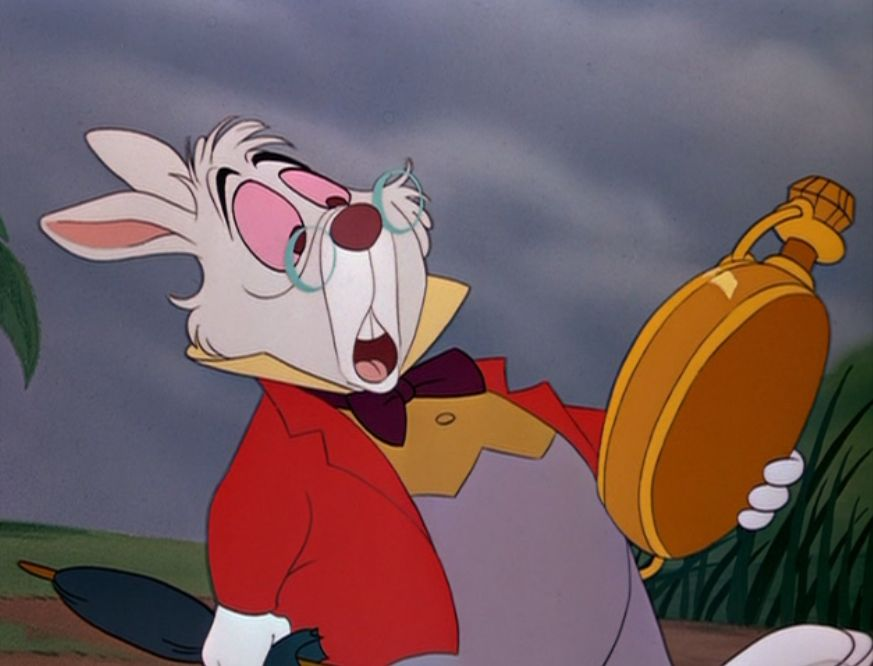
\includegraphics[scale=0.5]{rabbit.jpg} 
\end{center}
\caption{Во сколько, говоришь, домашку отправил?!}
\end{figure}

\subsection{}
\renewcommand{\theequation}{Eq. (\arabic{equation})}
\setcounter{equation}{0} 

\begin{equation}
\displaystyle \lim_{n \to \infty} \frac{n!}{\sqrt{2\pi n}*\left(\frac{n}{e}\right)^n} = 1 
\end{equation}

\begin{equation}
\displaystyle \rho=\frac{1}{\displaystyle \overline{\lim_{n \to \infty}} \sqrt[n]{|a_n|} }
\end{equation}

\subsection{}
\newenvironment{refrot}{
\newcommand{\rr}[2]{\reflectbox{##1} \rotatebox{180}{##2}}
}{}
\begin{refrot}
\rr{Дураками называют тех, кто выбирает нелегкий путь.}{Чеширский кот}
\end{refrot}

\subsection{Еще команда: чтобы крыша не поехала}
\newcommand{\sbh}[1]{\ensuremath{\displaystyle \hat\sigma_{\hat\beta_#1}^2}}
\sbh{1}, \sbh{0}

\end{document}
